\documentclass[preprint,12pt,authoryear]{elsarticle}
\usepackage{amsmath,amssymb,booktabs,array,graphicx,float,placeins,setspace,tabularx}
\usepackage[T1]{fontenc}
\usepackage[utf8]{inputenc}
\usepackage{lmodern,microtype}
\usepackage[colorlinks=true,citecolor=blue,linkcolor=blue,urlcolor=black]{hyperref}
\journal{International Journal of Forecasting}
\setlength{\emergencystretch}{2em}
\graphicspath{{figures/}}
\begin{document}
\begin{frontmatter}
\title{Forecast Evaluation with Constructed High-Frequency Targets: Information-Set Leakage and an African GDP Application}
\begin{abstract}
High-frequency forecast targets are often reconstructed from lower-frequency macroeconomic data. We show that forecast evaluation can become infeasible when a final-vintage disaggregated path is also treated as lagged information that was observable at historical forecast origins. For linear temporal-disaggregation procedures such as Denton, pre-origin monthly values can inherit nonzero weights on annual benchmarks that were not yet released. We formalize an information-set admissibility condition and study its consequences in two Monte Carlo designs plus a pure-noise placebo. In a modest current-state-signal design, publication-lagged information reveals short-horizon value that the retrospective final-vintage design largely suppresses. In a separate persistent-state stress calibration, chosen only to reproduce the direction of the empirical long-horizon reversal, mean 12-month relative RMSFE is 0.9962 under retrospective final-vintage information but 1.0122 under publication-lagged information. The placebo remains approximately neutral. The African application uses 21.30 million news records for 54 economies. A retrospective specification yields a favorable 12-month news comparison (relative RMSFE 0.9961), which becomes 1.0048 after forecast-origin GDP histories and training outcomes are constrained by publication timing. A modest one-month signal remains under a parsimonious benchmark (0.9964), but its raw bootstrap interval includes zero and it is not significant against a 159-series factor benchmark. The contribution is methodological: target construction, vintage status, release timing, and benchmark information are part of forecast design, not preprocessing details.
\end{abstract}
\begin{keyword}
forecast evaluation \sep constructed targets \sep real-time data \sep temporal disaggregation \sep information leakage \sep text-as-data
\par\medskip\textit{JEL classification:} C53; C82; E37; O55.
\end{keyword}
\end{frontmatter}
\singlespacing

\section{Introduction}
Forecast evaluation is meaningful only relative to the information that a forecaster could have observed at each historical origin. This principle is well established for revised macroeconomic data \citep{croushorestark2001,croushore2006}, but it has an additional implication when the forecast target itself is constructed at a higher frequency than the underlying official statistic. A final-vintage monthly or quarterly path may be perfectly acceptable as an ex post scoring target. The same path is not automatically admissible as a historical regressor, however, because a temporal-disaggregation operator can embed annual benchmarks that were released only later.\footnote{The distinction is between the object used for ex post scoring and the information set available at the forecast origin. Scoring a historical forecast against a subsequently revised outcome is not itself a look-ahead violation; the problem arises when information embodied in that later outcome is allowed to enter historical regressors or recursive estimation.}

This distinction matters increasingly for forecasting with alternative data. News, web prices, satellite indicators, payments data, and other high-frequency signals are often evaluated against official macroeconomic variables observed at lower frequency. When the official series is interpolated or benchmarked to match the alternative data, it is tempting to treat the resulting high-frequency history as if it were observed. Doing so changes the forecaster's information set and can change both the estimated benchmark and the apparent incremental value of the alternative signal.

We study this problem formally, in simulation, and in an African GDP application. The empirical setting contains 54 economies, an annual series supplied as ``GDP (PPP)-WEO,'' and a monthly Growth/Real Economy (GRE) news signal constructed from 21.30 million retained article records across 851 sources. The annual GDP series is converted to a monthly activity proxy using first-difference Denton benchmarking. The key design question is not whether the final-vintage monthly proxy can be used to score forecasts; it can. The question is whether its historical monthly values may enter lagged regressors and recursive training before the annual benchmarks that determine them would have been available.

The paper makes three contributions. First, we state a general information-set admissibility condition for forecasts that use linearly disaggregated targets. If pre-origin constructed values place nonzero weight on unreleased low-frequency benchmarks, the resulting exercise is retrospective rather than pseudo-out-of-sample. The sign of the distortion is not predetermined because both the benchmark and augmented model are affected. Second, two Monte Carlo designs show that the sign and horizon location of the distortion are not fixed. A modest current-state-signal design shows that retrospective final-vintage information can suppress feasible short-horizon value, while a persistent-state stress calibration shows that the retrospective design can also generate the same apparent long-horizon gain/loss reversal observed in the African application. The stress calibration is an existence result, not an estimated mechanism, and a pure-noise placebo remains approximately neutral. Third, the African application provides an empirical audit in which the correction changes the substantive conclusion: an apparent 12-month GRE advantage disappears after publication timing is enforced.

These contributions address two research questions. First, under what conditions does temporal disaggregation make a constructed high-frequency target inadmissible as historical forecast information? Second, how much can enforcing that admissibility condition change the measured incremental value of a fixed alternative-data predictor? Keeping these questions separate is important: the first is a methodological identification problem, whereas the second is an empirical forecast-evaluation problem.

The corrected empirical result is deliberately secondary. Under the baseline publication-lag rule, GRE reduces one-month RMSFE by about 0.36 percent and MAE by about 1.0 percent, but the raw RMSFE bootstrap interval includes zero, only 33 of 54 economies improve, and the incremental effect is not statistically persuasive against a wide 159-series factor benchmark. Exact-text deduplication leaves the short-horizon result similar, while direct information-staleness and revision regressions do not establish a strong economic mechanism. These qualifications are central rather than inconvenient: they show why the paper should be read as a contribution to forecast-evaluation design, not as evidence of universal news-based GDP forecast superiority.

The remainder of the paper is organized as follows. Section 2 develops the target-construction and information-set framework and documents the GRE measurement system. Section 3 sets out the recursive forecast design and Monte Carlo evidence. Section 4 presents the African GDP application, including the target-information audit, dependence-robust inference, measurement diagnostics, and data-rich benchmark. Section 5 discusses the implications, limitations, and replication scope.

\section{Constructed targets, text measurement, and information sets}
\subsection{Forecast evaluation, vintages, and alternative data}
The distinction between latest-available and real-time data has a long history in forecast evaluation. \citet{croushorestark2001} construct vintage-specific snapshots of macroeconomic information and show that revisions can alter forecasting conclusions. \citet{croushore2006} emphasizes that the forecaster's information set and the choice of ex post ``actual'' are separate objects: latest-vintage outcomes can be useful for evaluation, but latest-vintage historical regressors do not reproduce the problem faced in real time. This paper applies that logic to a less studied case in which the high-frequency target itself is generated by temporal disaggregation. If future annual totals help determine earlier monthly values, leakage can enter through the benchmark history even when the alternative predictor is dated correctly.

The problem is distinct from ordinary look-ahead in predictor scaling. It arises from the accounting constraint used to construct the target and therefore affects both lagged dependent variables and the timing at which training outcomes become usable. Our publication-lagged reconstruction does not create historical data vintages that are unavailable in the source archive; instead, it prevents annual years that had not yet been released under a stated convention from shaping the forecast-origin monthly path. This partial correction is deliberately separated from a fully real-time-vintage claim.

The text-as-data literature emphasizes that preprocessing, classification, and aggregation choices are part of the empirical design of a textual variable \citep{gentzkow2019}. Newspaper-based measures of policy uncertainty, geopolitical risk, and international uncertainty illustrate the value of transparent and replicable text rules \citep{baker2016,caldara2022,ahir2022}. Forecasting imposes a stronger test than descriptive association: a textual variable must reduce genuinely out-of-sample loss relative to the information already embedded in the benchmark.

Recent work in the \emph{International Journal of Forecasting} is particularly relevant. \citet{adaemmer2025} show that textual information can improve real-time macroeconomic tail-risk forecasts after conditioning on a large conventional information set. \citet{seo2025} constructs sector-specific textual indicators and embeds them in a text-enhanced factor model, providing direct evidence that economic organization of news can matter for forecast performance. \citet{zheng2024} combines textual and macroeconomic data in GDP nowcasting, while \citet{ardia2026} studies target-oriented construction of text-based indices. Together, these contributions show that the value of text-based forecasting research lies not only in the size of a forecast gain but also in how textual information is economically organized, benchmarked, and evaluated out of sample. The present paper is closest in spirit to that measurement-and-evaluation perspective. GRE is not optimized against GDP forecast loss: its vocabulary and scoring rule are fixed by economic semantics before forecast evaluation. The additional complication in the African application is that the comparable monthly activity target must itself be constructed from lower-frequency official benchmarks, making target measurement part of the forecast-evaluation problem.

A second recent IJF contribution, \citet{abeyie2026}, emphasizes that full article text and validated linguistic structure can improve text-based forecast models relative to headline-only representations. GRE likewise uses both normalized headline and body text, but retains an intentionally interpretable rule-based mapping. The objective is not to maximize predictive complexity; it is to determine whether a transparent real-economy news measure survives a demanding out-of-sample design.

The inferential design also draws on the panel forecast-evaluation literature. \citet{qu2024} show that forecast comparisons with panel data can exploit both the time-series and cross-sectional dimensions but must account for dependence to avoid severe size distortions. \citet{akgun2024} develop equal-predictive-ability procedures for panels under weak and strong cross-sectional dependence. Related work shows that strong dependence in loss differentials can sharply reduce the power of conventional predictive-accuracy tests \citep{coroneo2025}. We therefore report target-month HAC inference, cross-section-preserving moving-block bootstrap intervals, and a complementary two-way cluster-robust covariance calculation for the Clark--West adjusted loss differential. The latter is not presented as a substitute for the formal panel EPA statistics in those papers; it is a transparent robustness calculation that allows dependence along both country and target-month dimensions.

Data-rich forecasting provides the natural benchmark for claims about alternative information. Diffusion-index and factor methods summarize common variation in large predictor sets \citep{stockwatson2002}; recent evidence continues to examine the conditions under which factor augmentation improves forecasts \citep{bae2024}. Real-time nowcasting emphasizes the sequential arrival of heterogeneous information and the need to discipline forecasts by the information set available at each origin \citep{giannone2008,banbura2013,bok2018}. Because both the news signal and the activity proxy used here are monthly, a genuine MIDAS design would require an additional higher-frequency predictor set; introducing an artificial mixed frequency would not provide a meaningful benchmark. We therefore strengthen the benchmark set using no-change, pooled autoregressive, country-specific autoregressive, and common-factor specifications within the observed monthly information set.

Forecast combination provides a complementary operational perspective. Simple averages can be useful when estimated combination weights are unstable \citep{timmermann2006,stockwatson2004}. We therefore retain a fixed 50/50 combination of the statistical benchmark and the GRE-augmented forecast as a deployment diagnostic rather than an optimized model.

\subsection{News measurement in the African application}
The source registry contains 851 distinct newspaper and digital-news outlets spanning all 54 African economies. The registry records outlet name, country, publication language, and website. Source depth is intentionally heterogeneous: the median country has 13 registered outlets, with counts ranging from 2 to 66. The registry is multilingual, with substantial English- and French-language coverage, dedicated Arabic- and Portuguese-language sources, and additional national and regional languages as well as multilingual outlets. Registered-source counts are not interpreted as monthly availability; websites can enter or leave the accessible archive over time.

Articles are collected through a controlled monthly web-scraping workflow organized by country, outlet, and calendar month. Each source yields article titles and body text. Collection quality is assessed at the newspaper-month level. When retrieval falls at least 20 percent below the preceding month, the source is retried through scheduled passes. Only the strongest successful scrape for an outlet-month is retained; repeated attempts are never concatenated. The collection stage also applies cross-source duplicate checks, and incomplete or failed source-months remain distinguishable from observed months with no qualifying real-economy content. This design limits artificial variation caused by temporary website failures, repeated requests, or partial collection.

The frozen analytical archive contains 21,303,573 retained article records from January 2015 through December 2025, of which 5,896,776 satisfy the economic-relevance criterion. It contains 7,127 country-month observations; 6,488 have at least 100 retained articles, and the median country-month contains 1,039 records. The unit of measurement is an article record rather than an inferred independent news event. Cross-source screening reduces duplication but cannot eliminate all syndicated or edited copies. A reconstructed exact-text diagnostic removes 497,091 repeated records, or 2.33 percent of the frozen archive, including 186,379 cross-outlet copies. This diagnostic quantifies residual duplication without treating translated, edited, or substantively related stories as mechanically identical events.\footnote{The deduplication exercise is intentionally conservative: only exact decoded text matches within a country-month are collapsed. Rewrites, translations, syndicated stories with edits, and semantically similar reports remain separate records. The exercise therefore tests exact-copy sensitivity rather than semantic story duplication.}

Figure~\ref{fig:gre_descriptive} reports the cross-country median and interquartile range of GRE. Coverage varies over time, which is why the empirical analysis reports separate minimum-article robustness checks rather than assuming a homogeneous media environment.

\begin{figure}[htbp]
\centering
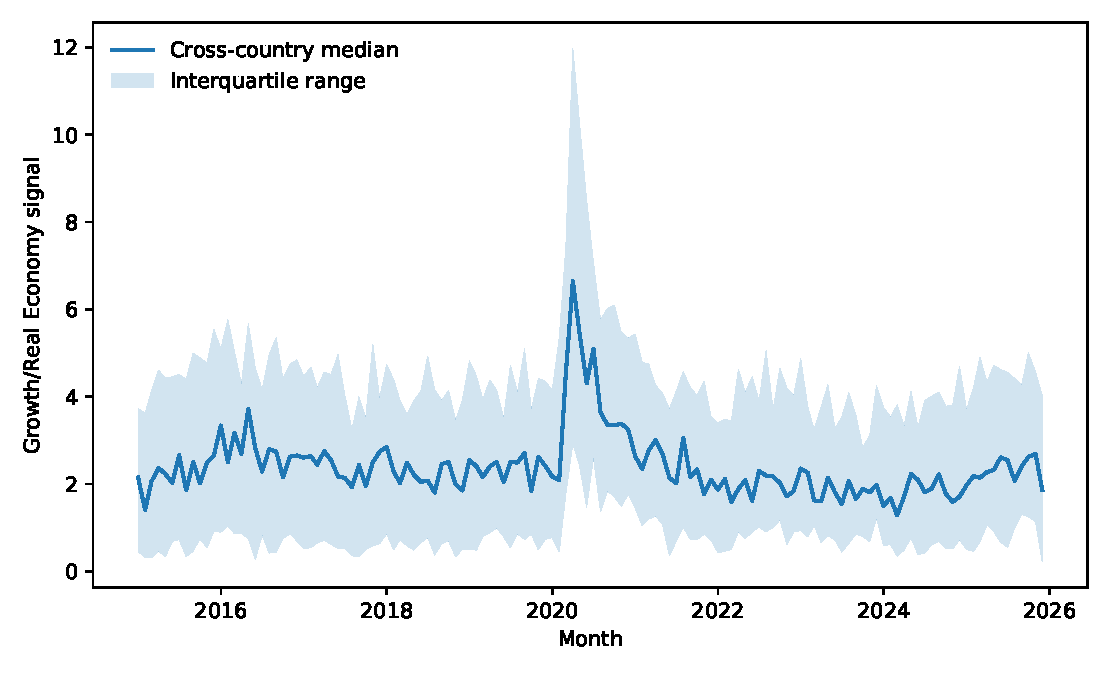
\includegraphics[width=0.82\textwidth]{Figure_0_GRE_Descriptive.pdf}
\caption{Cross-country distribution of the Growth/Real Economy news signal, 2015--2025. The line reports the monthly median and the shaded region the interquartile range across available country observations.}
\label{fig:gre_descriptive}
\end{figure}

As a simple archive-depth diagnostic, GRE is regressed on log retained article volume over the 6,488 country-months with at least 100 articles. The coefficient is 0.103 with country fixed effects ($p=0.656$) and 0.100 after adding full month fixed effects ($p=0.713$). These estimates do not establish representativeness of the news archive, but they provide little evidence that GRE moves mechanically with article volume within countries.

Let $x_i$ denote normalized headline and body text for article $i$. Economic relevance is
\begin{equation}
R_i=\mathbf{1}\{x_i\text{ matches the economic-relevance dictionary}\}.
\label{eq:relevance}
\end{equation}
Articles that fail this screen receive zero risk score but remain in the country-month denominator. This preserves the prevalence of economically relevant reporting relative to the complete observed news flow.

The target-specific activation indicator is
\begin{equation}
G_i=\mathbf{1}\{x_i\text{ activates the Growth/Real Economy dictionary}\}.
\label{eq:growthdomain}
\end{equation}
The frozen activation lexicon is intentionally compact. In English it contains recession, slowdown, contraction, unemployment, and layoffs, together with the corresponding French and Portuguese terms used in the production dictionary. Broader macroeconomic terms such as GDP and growth belong to the preceding economic-relevance screen rather than the GRE activation rule. This separation keeps target-specific activation narrow and auditable; the complete frozen dictionaries are reproduced in the replication documentation.\footnote{The GRE activation vocabulary is fixed before the forecasting exercise and is not selected by searching over alternative term sets for the lowest forecast loss. Ex post dictionary selection would create a distinct form of specification search and would weaken the interpretation of subsequent predictive-accuracy tests.}

Relevant articles receive an ordinal severity score. Let $\mathcal K_i\subseteq\{1,2,3,4\}$ contain the severity tiers matched in article $i$:
\begin{equation}
S_i=\begin{cases}
0,&R_i=0,\\
\max(\{1\}\cup\mathcal K_i),&R_i=1.
\end{cases}
\label{eq:severity}
\end{equation}
Tier 1 represents background or mild pressure; tier 2 material deterioration; tier 3 severe disruption; and tier 4 extreme or systemic real-economy stress. The scale is ordinal and is not interpreted as a recession probability.

Textual prominence is summarized by a headline cue $T_i$, a body-length indicator $L_i$ for at least 1,200 normalized characters, and an indicator $M_i$ for economically dense content activating at least two domains in the underlying taxonomy. The fixed weight is
\begin{equation}
W_i=\operatorname{clip}(1+0.5T_i+0.2L_i+0.3M_i,1,2),
\label{eq:weight}
\end{equation}
where $\operatorname{clip}(x,a,b)=\min\{\max(x,a),b\}$. These coefficients are part of the frozen production rule; they are not estimated from GDP or tuned to minimize forecast loss. Method consistency is enforced operationally through fixed scoring rules and input-method checks before new country-month observations are joined to the historical series. The article-level architecture also counts a qualifying article at most once within a given economic domain, so repeated keyword mentions do not mechanically increase its domain contribution. The empirical robustness analysis therefore keeps the baseline measurement rule fixed and evaluates exact-text duplication, article-volume thresholds, signal transformations, tail caps, and theory-motivated falsification domains rather than conducting alternative article-level re-scoring. These exercises assess the robustness of the frozen baseline signal to corpus- and signal-level choices; they do not constitute a sensitivity analysis of the underlying dictionary, severity map, or emphasis coefficients.

The article-level contribution to GRE is
\begin{equation}
Q_i=R_iG_iS_iW_i.
\label{eq:article}
\end{equation}
An economically relevant article about a different domain has $G_i=0$ and contributes zero to GRE. This feature is what differentiates the target-specific signal from broad AERI.

\begin{table}[htbp]
\centering\small
\caption{Construction of the Growth/Real Economy news signal}
\label{tab:construction}
\begin{tabularx}{\textwidth}{p{0.19\textwidth}X}
\toprule
Stage & Definition and interpretation \\
\midrule
Economic relevance $R_i$ & Indicator that normalized article text contains economically relevant content. Articles failing this screen contribute zero to the signal but remain in the country-month denominator. \\
Real-economy activation $G_i$ & Indicator that the article activates the frozen Growth/Real Economy dictionary: recession, slowdown, contraction, unemployment, layoffs, and the corresponding French and Portuguese activation terms. Broader GDP/growth vocabulary belongs to the economic-relevance screen rather than this target-specific activation rule. \\
Severity $S_i$ & Ordinal score for relevant articles: 1 = background or mild pressure; 2 = material deterioration; 3 = severe disruption; 4 = extreme or systemic real-economy stress. The highest matched tier applies. \\
Textual emphasis $W_i$ & $\operatorname{clip}(1+0.5T_i+0.2L_i+0.3M_i,1,2)$, where $T_i$ marks headline emphasis, $L_i$ marks at least 1,200 normalized characters, and $M_i$ marks economically dense multi-domain content. \\
Article contribution $Q_i$ & $Q_i=R_iG_iS_iW_i$. Only economically relevant articles that activate the real-economy domain contribute positive weight. \\
Country-month signal $GRE_{ct}$ & $100N_{ct}^{-1}\sum_{i\in\mathcal A_{ct}}Q_i$, where $N_{ct}$ is the total number of retained articles. The signal therefore reflects both the prevalence and the intensity of real-economy risk reporting. \\
\bottomrule
\end{tabularx}
\end{table}

\begin{table}[htbp]
\centering\scriptsize
\caption{Illustrative article-level mapping into the Growth/Real Economy signal}
\label{tab:worked_example}
\begin{tabularx}{\textwidth}{p{0.32\textwidth}cccccX}
\toprule
Stylized article content & $R_i$ & $G_i$ & $S_i$ & $W_i$ & $Q_i$ & Interpretation \\
\midrule
``Manufacturing output contracts sharply; factories announce layoffs and demand weakens'' & 1 & 1 & 3 & 2.0 & 6.0 & Economically relevant, activates the real-economy domain, severe language, and high textual emphasis. \\
``Foreign-exchange reserves decline while the currency comes under pressure'' & 1 & 0 & -- & -- & 0 & Economically relevant but does not activate the Growth/Real Economy domain, so it does not enter this signal. \\
Sports or entertainment article with no economic content & 0 & 0 & 0 & -- & 0 & Retained in the monthly article denominator but contributes zero to the numerator. \\
\bottomrule
\end{tabularx}
\vspace{0.3em}
\begin{minipage}{0.96\textwidth}\footnotesize\textit{Notes:} Examples are stylized illustrations, not quotations from the archive. For the first row, $W_i$ reaches its upper bound when all three emphasis indicators are active.\end{minipage}
\end{table}


For country $c$ and month $t$, let $\mathcal A_{ct}$ denote the retained article set and $N_{ct}=|\mathcal A_{ct}|$. The GRE signal is
\begin{equation}
GRE_{ct}=\frac{100}{N_{ct}}\sum_{i\in\mathcal A_{ct}}R_iG_iS_iW_i.
\label{eq:gre}
\end{equation}
The full article count remains in the denominator. Consequently, GRE increases when real-economy risk reporting becomes more prevalent, more severe or prominent, or both. Define
\begin{equation}
B^G_{ct}=\frac{\sum_iR_iG_i}{N_{ct}}, \qquad
\overline{SW}^{G}_{ct}=\frac{\sum_iR_iG_iS_iW_i}{\sum_iR_iG_i}.
\end{equation}
Whenever the conditional denominator is positive,
\begin{equation}
GRE_{ct}=100B^G_{ct}\overline{SW}^{G}_{ct}.
\label{eq:decomp}
\end{equation}
This decomposition separates the breadth of real-economy reporting from its conditional severity and prominence.

The closest construction-based comparator is broad AERI,
\begin{equation}
AERI_{ct}=\frac{100}{N_{ct}}\sum_{i\in\mathcal A_{ct}}R_iS_iW_i.
\label{eq:aeri_comp}
\end{equation}
The only difference is the absence of $G_i$. AERI therefore asks whether general economic-risk reporting is enough, whereas GRE asks whether restricting the same scored news flow to the real-economy domain yields a more useful forecasting variable. At the forecasting stage, Inflation Risk and FX/External Risk are also reported as economically motivated, non-matched falsification comparators. These additional domains do not enter GRE construction and are not used to select or tune the GRE signal.

\subsection{Annual GDP, temporal disaggregation, and information-set admissibility}
The low-frequency activity panel covers all 54 African economies from 2015 through 2025. The source workbook supplied for this study labels the annual series ``GDP (PPP)-WEO.'' The replication package archives the exact workbook as supplied on 13 September 2026 and a cleaned country-year extract. The workbook does not embed a WEO publication-release identifier or historical vintage. We therefore do not infer one. Throughout the paper these annual observations are described as final-vintage WEO-labelled benchmarks. This treatment resolves the distinction between data provenance and historical availability: the provider label is recorded exactly as supplied, while vintage-real-time availability is not claimed.\footnote{The phrase ``WEO-labelled'' refers only to the label contained in the supplied workbook. Because the workbook does not identify a specific IMF World Economic Outlook release, no exact WEO vintage is inferred or attributed in the empirical analysis.}

Comparable official monthly GDP releases are not available for the full African panel. We construct a monthly GDP-PPP \emph{activity proxy} using additive first-difference Denton temporal disaggregation \citep{denton1971,imfqna2017}. For country $c$, let $Y_{cy}$ denote annual GDP-PPP and let $G^{F}_{ct}$ denote the final-vintage monthly proxy. The construction solves
\begin{equation}
\min_{\{G^{F}_{ct}\}}\sum_{t=2}^{T}(G^{F}_{ct}-G^{F}_{c,t-1})^2
\quad\text{subject to}\quad
\sum_{m=1}^{12}G^{F}_{c,y,m}=Y_{cy}\quad\forall y.
\label{eq:denton}
\end{equation}
The realized evaluation target is twelve-month growth,
\begin{equation}
y^{F}_{ct}=100[\log G^{F}_{ct}-\log G^{F}_{c,t-12}].
\label{eq:gdp12}
\end{equation}
The superscript $F$ is important: this is an ex post final-vintage outcome proxy, not a monthly national-accounts series that would have been observed in real time.

For a fixed sample, Denton benchmarking is a linear mapping from annual benchmarks to the constructed monthly vector. Write the final-vintage annual vector as $Y^F$ and the corresponding monthly path as
\begin{equation}
G^F=H Y^F,
\label{eq:linear_operator}
\end{equation}
where $H$ is the matrix implied by the quadratic minimization and annual aggregation constraints. At forecast origin $t$, partition $Y^F=(Y_t^A,Y_t^U)$ into annual benchmarks that are available and unavailable under the historical information rule, and partition the columns of $H$ conformably.

\paragraph{Information-set admissibility.}
A constructed historical path is admissible at origin $t$ only if the rows used by the forecasting model satisfy $H_{\leq t,U}=0$, or if an equivalent one-sided reconstruction is performed using only $Y_t^A$. If $H_{\leq t,U}\neq0$, then $G^F_{\leq t}$ depends on annual information not measurable with respect to the feasible forecast-origin information set. A recursive forecast that uses those values as lagged regressors, or admits targets into estimation before the annual information needed to construct them would have been released, is retrospective rather than pseudo-out-of-sample. The direction of the resulting forecast-loss distortion is generally ambiguous because both the benchmark information set and the estimated augmentation can change.

This condition extends the real-time-data logic of \citet{croushorestark2001} to constructed targets. It is not a claim that temporal disaggregation is inappropriate. The issue is the role assigned to the disaggregated path inside the forecast experiment. A final-vintage path can be a legitimate realized outcome while still being inadmissible as historical forecast-origin information.

Figure~\ref{fig:leakage} summarizes the distinction. The upper path is valid for retrospective description and ex post scoring but becomes inadmissible if the full constructed history is fed into a historical forecast origin. The lower path separates origin-available GDP information from the final-vintage outcome that is observed only later for evaluation.

\begin{figure}[htbp]
\centering
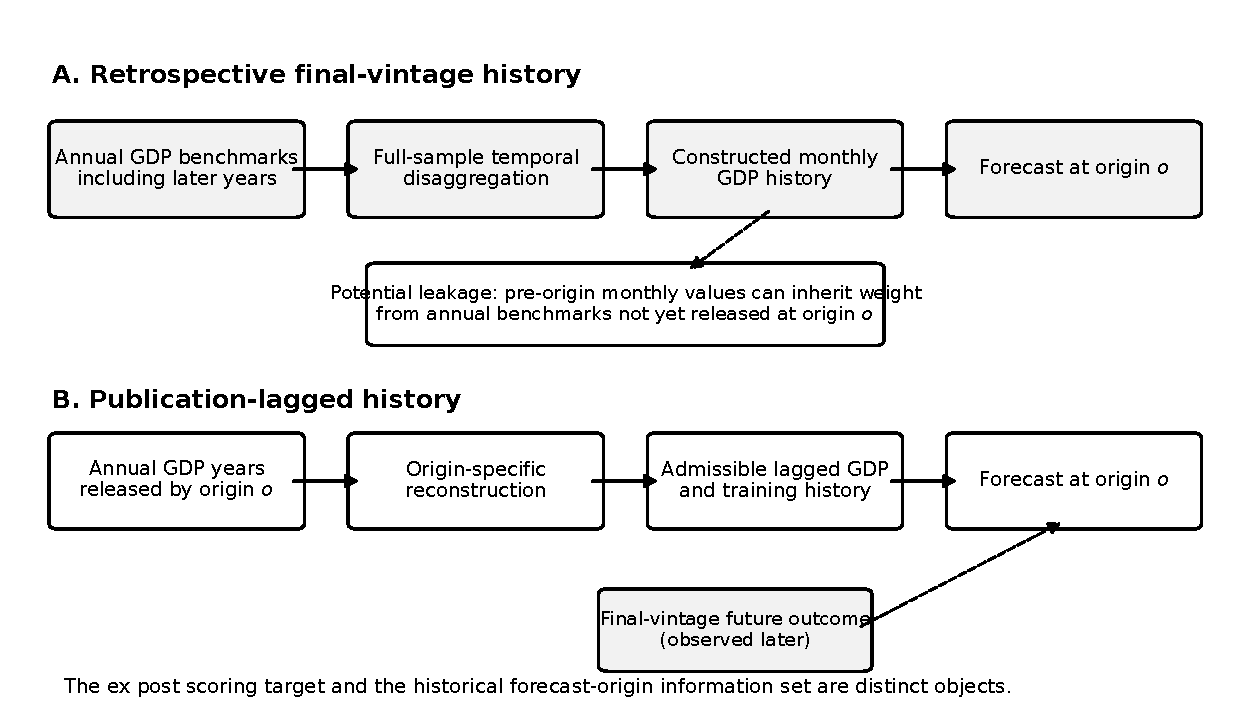
\includegraphics[width=0.96\textwidth]{Figure_Target_Information_Leakage.pdf}
\caption{Target-information leakage in retrospective versus publication-lagged forecast construction.}
\label{fig:leakage}
\begin{singlespace}\footnotesize\textit{Notes:} The retrospective path may allow unreleased annual benchmarks to influence pre-origin monthly values through temporal disaggregation. The publication-lagged path reconstructs lagged GDP and training information using only annual years permitted at the forecast origin. A final-vintage future outcome can still be used later for scoring without being treated as information available at the origin.\end{singlespace}
\end{figure}

\subsection{Publication-lagged reconstruction}
Using $G^{F}_{ct}$ directly as a lagged predictor would allow future annual benchmarks to shape the historical monthly path. We therefore reconstruct the GDP information set separately at every forecast origin $s$. Under the baseline release rule, the latest annual benchmark year permitted at origin $s$ is
\begin{equation}
a(s)=
\begin{cases}
\operatorname{year}(s)-1, & \operatorname{month}(s)\geq 5,\\
\operatorname{year}(s)-2, & \operatorname{month}(s)<5.
\end{cases}
\label{eq:availyear}
\end{equation}
Only annual benchmarks through $a(s)$ are supplied to the Denton problem. For months after December of $a(s)$ and up to the forecast origin, the monthly path is extrapolated using the constant log-monthly rate implied by the two most recent permitted annual totals,
\begin{equation}
r_{c,s}=\frac{1}{12}\left[\log Y_{c,a(s)}-\log Y_{c,a(s)-1}\right],
\label{eq:extraprate}
\end{equation}
with a zero trend if only one annual benchmark is available. This produces an origin-specific path $G^{I(s)}_{ct}$ and corresponding lagged twelve-month growth $y^{I(s)}_{ct}$. The same release rule governs recursive training: an outcome dated in calendar year $y$ is eligible for estimation only from May of $y+1$. We repeat the complete exercise with July and November release months.\footnote{The May rule is an explicit operational convention, not a claim that all 54 economies publish annual GDP on a common date. The July and November exercises are intended to show whether the conclusions depend on a relatively early annual-information assumption.}

The rule is intentionally transparent and conservative, but it does not solve historical revision uncertainty. Annual observations through $a(s)$ are still taken from the final-vintage replication file rather than from archived contemporaneous releases. Consequently, the design prevents mechanical use of future \emph{years} in the forecast information set, but it does not remove information embedded in later revisions to already released years. We therefore avoid the term ``real-time'' and use ``publication-lagged final-vintage'' throughout.
\section{Forecast design and simulation evidence}
\subsection{Publication-lagged forecast design and inference}
Country membership and text scaling are determined before evaluation. GRE and comparator text signals are standardized within country using January 2015--December 2018 means and standard deviations, which are frozen before the January 2020 evaluation start. No country is selected using a news--GDP correlation, coefficient sign, or evaluation-period forecast performance.

For horizon $h$, the benchmark is
\begin{equation}
y^{F}_{c,t+h}=\alpha_c+\sum_{j=0}^{2}\phi_{j,h}y^{I(t)}_{c,t-j}
+\sum_{m=2}^{12}\delta_{m,h}\mathbf{1}\{M_{t+h}=m\}+u_{c,t+h},
\label{eq:benchmark}
\end{equation}
where the three GDP-growth lags are reconstructed from the information set available at forecast origin $t$. The GRE specification adds standardized GRE measured at $t$. Parameters are re-estimated recursively over expanding samples subject to the target-release rule. Target dates span January 2020--December 2025, and forecast horizons are 1, 3, 6, and 12 months. Because the target-timing correction was introduced after the earlier 12-month specification had been examined, we report the complete horizon profile and do not relabel the one-month horizon as a newly pre-specified primary test.

\begin{table}[htbp]
\centering\scriptsize\singlespacing
\caption{Publication-lagged final-vintage forecasting design}
\label{tab:design}
\renewcommand{\arraystretch}{0.92}
\begin{tabularx}{\textwidth}{p{0.24\textwidth}X}
\toprule
Element & Implementation \\
\midrule
Country universe & Fifty-four African economies; membership is determined by pre-evaluation data availability only. \\
Annual GDP source & Author-supplied annual series labelled ``GDP (PPP)-WEO,'' 2015--2025. The replication copy is frozen as supplied on 13 September 2026. The workbook does not identify the underlying WEO publication vintage, so the annual values are treated as final-vintage data rather than historical real-time vintages. \\
Realized evaluation target & Twelve-month growth of a final-vintage monthly GDP-PPP proxy constructed by additive first-difference Denton and constrained to aggregate exactly to the annual benchmarks. This series is used only to score realized forecast outcomes. \\
Forecast-origin GDP information & At each forecast origin, lagged monthly GDP growth is reconstructed from annual benchmark years permitted by the release rule. Under the baseline rule, year $y$ becomes usable from May of $y+1$. Denton is applied only through the last permitted annual year; subsequent months up to the forecast origin are extrapolated using the log-monthly rate implied by the two most recent permitted annual totals. \\
Training-target availability & A realized target dated in calendar year $y$ enters recursive estimation only from May of $y+1$ under the baseline rule. \\
Text scaling & Country-specific GRE and comparator means and standard deviations are estimated over 2015--2018 and frozen before the January 2020 evaluation start. \\
Benchmark & Pooled country-fixed-effects autoregression using three publication-lagged GDP-growth lags and target-month seasonal indicators. GRE adds one standardized news regressor at the forecast origin. \\
Evaluation & Recursive target dates January 2020--December 2025 at 1-, 3-, 6-, and 12-month forecast horizons. The full horizon profile is reported; no new horizon is relabelled as pre-specified after inspection of the corrected results. \\
Release-timing sensitivity & Baseline May availability is repeated using July and November release conventions. \\
Inference & RMSFE, MAE, target-month HAC Clark--West inference, complementary two-way country--target-month covariance, Holm correction across horizons, cross-section-preserving moving-block bootstrap, and country-level RMSFE ratios. \\
\bottomrule
\end{tabularx}
\end{table}


Forecast accuracy is summarized by RMSFE and MAE. Nested comparisons use the Clark--West adjusted loss differential \citep{clarkwest2007}.\footnote{For nested models, estimating an additional coefficient can raise the augmented model's raw mean-squared forecast error even when the added predictor contains useful population information. The Clark--West adjustment corrects for this estimation-noise effect. Raw loss measures and adjusted-loss tests therefore answer related but distinct questions, which is why both are reported throughout.} The principal dependence-robust calculation averages the Clark--West differential across countries within target month and applies Newey--West HAC inference, with horizon-appropriate overlap lags. This procedure preserves the contemporaneous cross-section rather than treating country errors as independent. As a complementary diagnostic, we report observation-level two-way covariance clustered by country and target month, motivated by the panel forecast-comparison literature \citep{qu2024,akgun2024,coroneo2025}. We also apply Holm correction across the four horizons and use a moving-block bootstrap that resamples 12-month target-date blocks while preserving all countries within each selected month.\footnote{Resampling target dates rather than individual country observations preserves the contemporaneous cross-country dependence visible in the forecast-error panel. The 12-month block length also accommodates the overlap induced by the twelve-month growth target.}

Cross-sectional dependence remains substantial after the information correction. For the one-month benchmark, the balanced diagnostic panel contains 53 countries over 72 target months, the mean pairwise forecast-error correlation is approximately 0.442, and the corresponding Pesaran CD statistic is about 139.2. Dependence-aware inference is therefore necessary.

\subsection{Monte Carlo design}
The empirical audit establishes that information timing matters in this application, but a single application cannot show whether the issue is peculiar to one dataset. We therefore use two stylized Monte Carlo designs to isolate the information-set channel and to clarify what the simulation can, and cannot, establish. Each replication contains 54 economies and a monthly calendar from 2015 through 2025. Annual GDP follows a panel process with country-specific average growth, a common annual component, and idiosyncratic innovations. Annual flows are converted to monthly frequency using the same first-difference Denton operator used in the empirical application. Forecasts condition on three lags of twelve-month growth and country fixed effects. To isolate target-information treatment, the simulations use a fixed pre-evaluation estimation window and evaluate 2020--2025.

The first data-generating process is intentionally modest. The alternative-data variable measures the contemporaneous annual activity innovation with noise and contains no next-year innovation. Its scale is calibrated so that, under feasible publication timing, the one-month improvement is small and of the same order as the corrected empirical result. The second design is a \emph{persistent-state stress DGP}. It raises annual persistence and the signal-to-noise ratio specifically to ask whether retrospective final-vintage information can produce the direction of the empirical 12-month reversal. This second calibration is deliberately an existence demonstration. It is not fitted to the African data, it does not reproduce the full empirical horizon profile, and it is not used to claim that persistence is the empirical mechanism. A separate placebo replaces the signal with independent noise.

For every DGP, two information treatments are compared. The retrospective design supplies the complete final-vintage Denton history to the forecasting model. The publication-lagged design admits annual benchmark $y$ only from May of $y+1$ and extrapolates the most recent released annual information between releases, exactly as in the empirical baseline. We report 1,000 replications for each signal design and retain the pure-noise placebo as a falsification check.

\subsection{Monte Carlo results}
\begin{table}[htbp]
\centering
\small
\caption{Monte Carlo: target-information treatment and the horizon profile of text value}
\label{tab:simulation}
\resizebox{\textwidth}{!}{%
\begin{tabular}{@{}llrrr@{}}
\toprule
DGP & Design & $h$ & Mean relative RMSFE & Share with RMSFE gain \\
\midrule
Current-state signal & Retrospective final-vintage & 1 & 1.0002 & 39.0\% \\
Current-state signal & Publication-lagged & 1 & 0.9969 & 97.7\% \\
Current-state signal & Retrospective final-vintage & 3 & 1.0002 & 36.6\% \\
Current-state signal & Publication-lagged & 3 & 0.9973 & 96.5\% \\
Current-state signal & Retrospective final-vintage & 6 & 1.0002 & 39.2\% \\
Current-state signal & Publication-lagged & 6 & 0.9987 & 84.6\% \\
Current-state signal & Retrospective final-vintage & 12 & 1.0001 & 47.5\% \\
Current-state signal & Publication-lagged & 12 & 1.0025 & 47.6\% \\
\midrule
Persistent-state stress & Retrospective final-vintage & 12 & 0.9962 & 90.2\% \\
Persistent-state stress & Publication-lagged & 12 & 1.0122 & 35.1\% \\
\bottomrule
\end{tabular}}
\begin{singlespace}\footnotesize\textit{Notes:} 1,000 replications per DGP with 54 economies and a 2015--2025 monthly calendar. The current-state signal is calibrated to a modest feasible short-horizon effect and contains no next-year innovation. The persistent-state stress DGP deliberately increases persistence and signal-to-noise to test whether retrospective final-vintage information can reproduce the direction of the empirical 12-month reversal; it is an existence calibration, not an empirical mechanism estimate. A separate pure-noise placebo remains approximately neutral under both information treatments. Full horizon results for all three DGPs appear in the online supplement.\end{singlespace}
\end{table}


\begin{figure}[htbp]
\centering
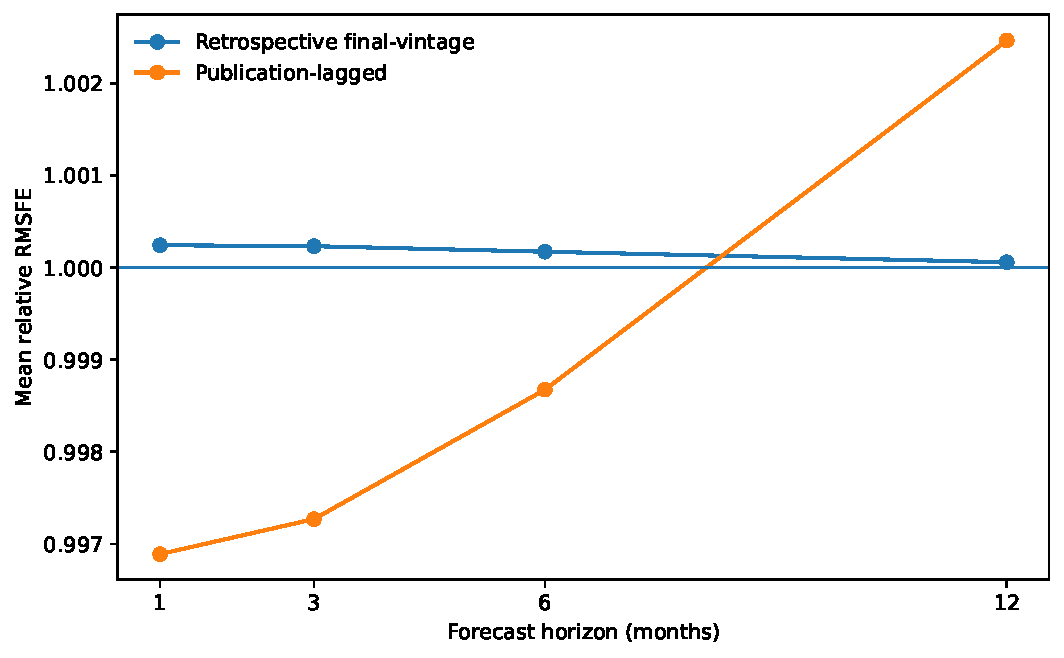
\includegraphics[width=0.76\textwidth]{Figure_Simulation_Horizon_Distortion.pdf}
\caption{Baseline Monte Carlo horizon profile under retrospective and publication-lagged target information.}
\label{fig:simulation}
\begin{singlespace}\footnotesize\textit{Notes:} Lines report mean relative RMSFE across 1,000 replications for the modest current-state-signal DGP. Values below one favor the text-augmented model. The persistent-state stress calibration is summarized in Table~\ref{tab:simulation} and reported fully in the online supplement.\end{singlespace}
\end{figure}

The two signal DGPs demonstrate different, complementary distortions. In the modest current-state design, publication-lagged information reveals short-horizon value that is almost completely suppressed by the retrospective specification. Mean one-month relative RMSFE is 0.9969 under publication-lagged information but 1.0002 under retrospective final-vintage information. At twelve months, the retrospective ratio is 1.0001 and the publication-lagged ratio is 1.0025. This design therefore validates the general proposition that information-set treatment can alter the magnitude and horizon profile of a plausible high-frequency signal, but it does \emph{not} reproduce the empirical long-horizon reversal.

The persistent-state stress calibration addresses that limitation explicitly. With deliberately high annual persistence and a stronger contemporaneous signal, mean 12-month relative RMSFE is 0.9962 under retrospective final-vintage information but 1.0122 under publication-lagged information. This matches the \emph{direction} of the African reversal, where 0.9961 becomes 1.0048 after publication timing is imposed. The stress DGP generates much larger short-horizon effects than the data, however, and is therefore not presented as a calibrated explanation of the empirical result. Its role is narrower: it establishes that an admissibility violation can, under plausible alternative persistence and signal-to-noise configurations, create an apparent long-horizon advantage that disappears once the information set is made feasible.\footnote{The stress parameters are chosen to demonstrate existence of the empirical-style reversal, not estimated from the African panel or tuned to match the full set of empirical moments. The simulation therefore supports the possibility of this distortion but does not identify the mechanism generating the observed African reversal.}

Taken together, the two designs explain why the sign of the admissibility distortion is intentionally left unrestricted. Final-vintage target information can mask a feasible short-horizon signal in one DGP and create an apparent long-horizon gain in another. The empirical application need not share the exact simulation mechanism for the information-set critique to hold. The pure-noise placebo remains approximately neutral, so the simulations do not imply that temporal disaggregation automatically manufactures predictive power for arbitrary variables.

\section{Empirical application: African GDP forecasting}
\subsection{Target-information audit}
Table~\ref{tab:target_audit} makes the look-ahead issue explicit. The earlier working design used the final-vintage Denton series both as the realized target and as lagged GDP information. That specification produced a 12-month relative RMSFE of 0.9961 with nominal Clark--West $p=0.033$. Once forecast-origin GDP lags are reconstructed from publication-permitted annual years and training outcomes are delayed until their assumed release date, the 12-month relative RMSFE becomes 1.0048 and the nominal long-horizon advantage disappears. The favorable evidence moves to the one- and three-month horizons.

\begin{table}[htbp]
\centering\small\singlespacing
\caption{Target-information audit: final-vintage lags versus publication-lagged lags}
\label{tab:target_audit}
\begin{tabularx}{\textwidth}{p{0.35\textwidth}rrX}
\toprule
Design & Horizon & Relative RMSFE & Interpretation \\
\midrule
Final-vintage monthly GDP treated as available at origin & 12 & 0.9961 & Retrospective diagnostic only; nominal CW $p=0.033$. \\
Publication-lagged GDP information set & 12 & 1.0048 & No long-horizon GRE gain; HAC CW $p=0.905$. \\
Publication-lagged GDP information set & 1 & 0.9964 & Modest short-horizon predictive content; HAC CW $p=0.0006$. \\
\bottomrule
\end{tabularx}
\vspace{0.35em}
\begin{minipage}{0.97\textwidth}\footnotesize\textit{Notes:} The first row reproduces the earlier working specification in which the final-vintage temporally disaggregated GDP proxy was also used as forecast-origin lag information. Because that monthly path incorporates annual benchmarks not available at historical origins, it is not used as pseudo-out-of-sample evidence in the revised paper. The corrected design uses the final-vintage series only as the realized outcome and reconstructs forecast-origin GDP information under explicit release lags.\end{minipage}
\end{table}


This reversal is substantively important. It shows why a constructed high-frequency target cannot be treated simultaneously as an ex post outcome and as if its final-vintage history had been observable to the forecaster. The retrospective final-vintage result is retained in the replication package only as an audit trail; it is not used to support the paper's predictive claim.

Figure~\ref{fig:empirical_reversal} displays the full horizon profile under both information treatments. The visual comparison makes clear that the correction is not a small adjustment to inference: it changes where the apparent predictive advantage occurs and reverses the sign of the 12-month comparison.

\begin{figure}[htbp]
\centering
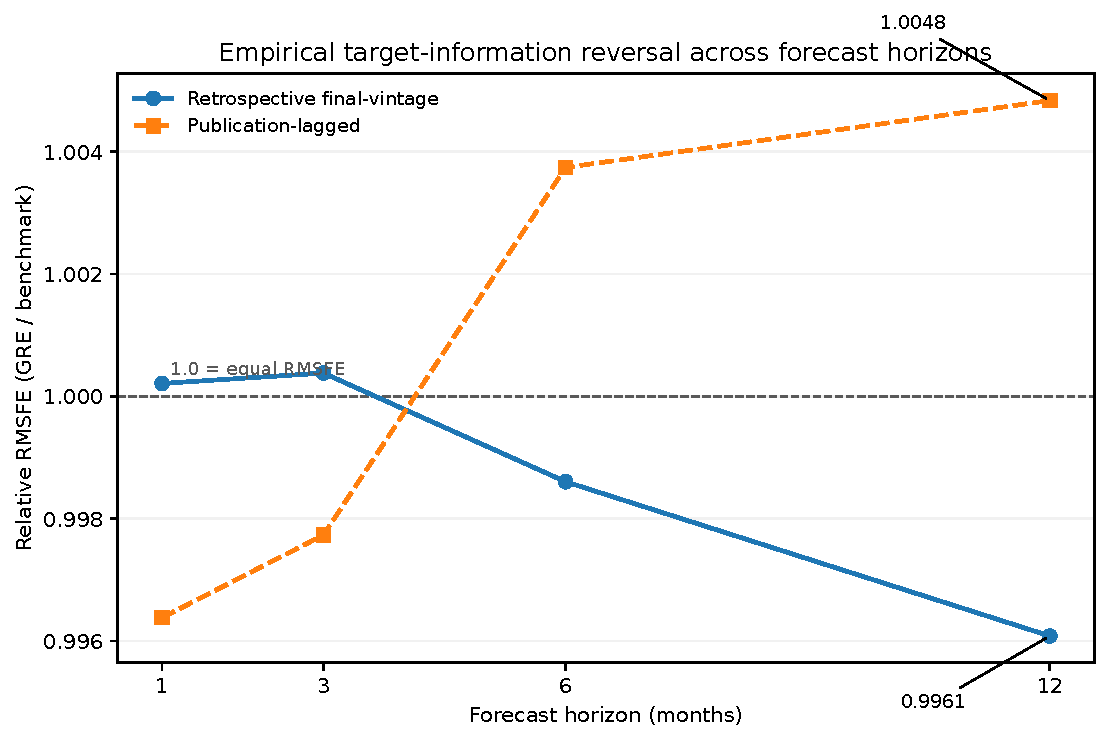
\includegraphics[width=0.82\textwidth]{Figure_Empirical_Horizon_Reversal.pdf}
\caption{Empirical horizon profile under retrospective final-vintage and publication-lagged information.}
\label{fig:empirical_reversal}
\begin{singlespace}\footnotesize\textit{Notes:} Relative RMSFE below one favors GRE. The retrospective specification uses the full final-vintage Denton history as lagged GDP information. The publication-lagged specification reconstructs forecast-origin GDP histories using only annual benchmark years permitted by the release rule.\end{singlespace}
\end{figure}

\subsection{Corrected horizon profile and release timing}
Table~\ref{tab:main_results} reports the publication-lagged forecast comparison. The central finding is that the information-timing correction changes the horizon profile rather than merely changing standard errors. At one month ahead, benchmark RMSFE is 8.375 and GRE RMSFE is 8.344, for relative RMSFE 0.9964. MAE falls from 5.441 to 5.385, giving relative MAE 0.9897. At three months, relative RMSFE is 0.9977 and relative MAE is 0.9928. At six and twelve months the RMSFE ratios rise above one, to 1.0037 and 1.0048, respectively.

\begin{table}[htbp]
\centering\scriptsize
\caption{Publication-lagged forecast performance of the GRE-augmented model}
\label{tab:main_results}
\resizebox{\textwidth}{!}{%
\begin{tabular}{rrrrrrrr}
\toprule
$h$ & Benchmark RMSFE & GRE RMSFE & Rel. RMSFE & Benchmark MAE & GRE MAE & HAC CW $p$ & Two-way $p$ \\
\midrule
1  & 8.375 & 8.344 & 0.9964 & 5.441 & 5.385 & 0.0006 & 0.053 \\
3  & 8.493 & 8.473 & 0.9977 & 5.523 & 5.483 & 0.041 & 0.084 \\
6  & 8.588 & 8.620 & 1.0037 & 5.513 & 5.529 & 0.878 & 0.869 \\
12 & 19.264 & 19.357 & 1.0048 & 7.028 & 7.114 & 0.905 & 0.872 \\
\bottomrule
\end{tabular}}
\vspace{0.35em}
\begin{minipage}{0.97\textwidth}\footnotesize\textit{Notes:} The dependent variable is final-vintage twelve-month GDP-PPP proxy growth. Forecast-origin GDP lags and the recursive training sample obey the baseline May release rule described in Table~\ref{tab:design}. Relative RMSFE below one indicates lower forecast loss. Holm adjustment across the four target-month HAC tests gives adjusted $p=0.0023$ at $h=1$ and $p=0.122$ at $h=3$. The corresponding two-way adjusted values are 0.211 and 0.253.\end{minipage}
\end{table}


At one month, target-month HAC Clark--West inference gives $p=0.0006$. The complementary two-way country--target-month value is $p=0.053$. Holm correction across the four HAC horizon tests gives adjusted $p=0.0023$ at one month and 0.122 at three months; the two-way adjusted values are larger. A 5,000-draw target-month moving-block bootstrap gives a one-sided Clark--West value of $p=0.037$. The raw percentage RMSFE improvement is about 0.36 percent, and its 95 percent bootstrap interval is approximately $[-0.50,1.44]$, so the magnitude remains imprecisely estimated even though the adjusted-loss evidence is favorable. Country-level RMSFE is lower with GRE in 33 of 54 economies, with a median country ratio of approximately 0.991.

The corrected evidence is therefore not a claim of large or universal forecast dominance. It indicates modest incremental information in GRE for forecasting the next few observations of twelve-month GDP growth when the conventional GDP information set is publication constrained.

The baseline May rule is not intended to assert an exact release date for every African economy. It is a transparent availability convention. Table~\ref{tab:release_timing} therefore repeats the entire origin-specific reconstruction using July and November of the following year. The one-month GRE result remains favorable under both more conservative rules. Relative RMSFE is 0.9969 under July availability and 0.9973 under November availability; relative MAE remains near 0.99. Target-month HAC values remain below 0.001, two-way values are 0.039 and 0.030, and bootstrap Clark--West values are 0.038 and 0.019. Between 31 and 33 of 54 countries have lower one-month RMSFE across the three release conventions.

\begin{table}[htbp]
\centering\small
\caption{Sensitivity of the one-month GRE result to annual-data release timing}
\label{tab:release_timing}
\resizebox{\textwidth}{!}{%
\begin{tabular}{lrrrrrr}
\toprule
Annual year $y$ usable from & Rel. RMSFE & Rel. MAE & HAC CW $p$ & Two-way $p$ & Bootstrap CW $p$ & Countries $<1$ \\
\midrule
May of $y+1$ & 0.9964 & 0.9897 & 0.0006 & 0.053 & 0.037 & 33/54 \\
July of $y+1$ & 0.9969 & 0.9894 & 0.0004 & 0.039 & 0.038 & 31/54 \\
November of $y+1$ & 0.9973 & 0.9910 & 0.0001 & 0.030 & 0.019 & 32/54 \\
\bottomrule
\end{tabular}}
\vspace{0.35em}
\begin{minipage}{0.97\textwidth}\footnotesize\textit{Notes:} Each row reconstructs the GDP information set and recursive training eligibility under the stated release convention. Bootstrap results use 5,000 moving-block replications with 12-month target-date blocks and preserve the contemporaneous country cross-section.\end{minipage}
\end{table}


This robustness matters because the paper does not possess archived release dates or historical annual data vintages for every country. The result is not tied to treating annual data as available immediately after year-end.

\subsection{Loss uncertainty, country breadth, and domain alignment}
At the one-month horizon, 82.6 percent of 5,000 moving-block replications imply a lower raw RMSFE under GRE. The 95 percent interval for the percentage RMSFE improvement is approximately $[-0.50,1.44]$, while the bootstrap Clark--West one-sided value is 0.037. The difference between raw-loss uncertainty and nested-model adjusted-loss inference is reported directly rather than resolved by selecting one statistic. Country-level evidence is similarly heterogeneous: 33 of 54 economies have lower RMSFE and 21 do not, although the median country ratio is approximately 0.991.

Figure~\ref{fig:country_heterogeneity} reports all country-level ratios rather than reducing that heterogeneity to a single count. The dispersion reinforces the interpretation that the pooled result is an average short-horizon signal, not a claim of uniform country-level forecast superiority.

\begin{figure}[p]
\centering
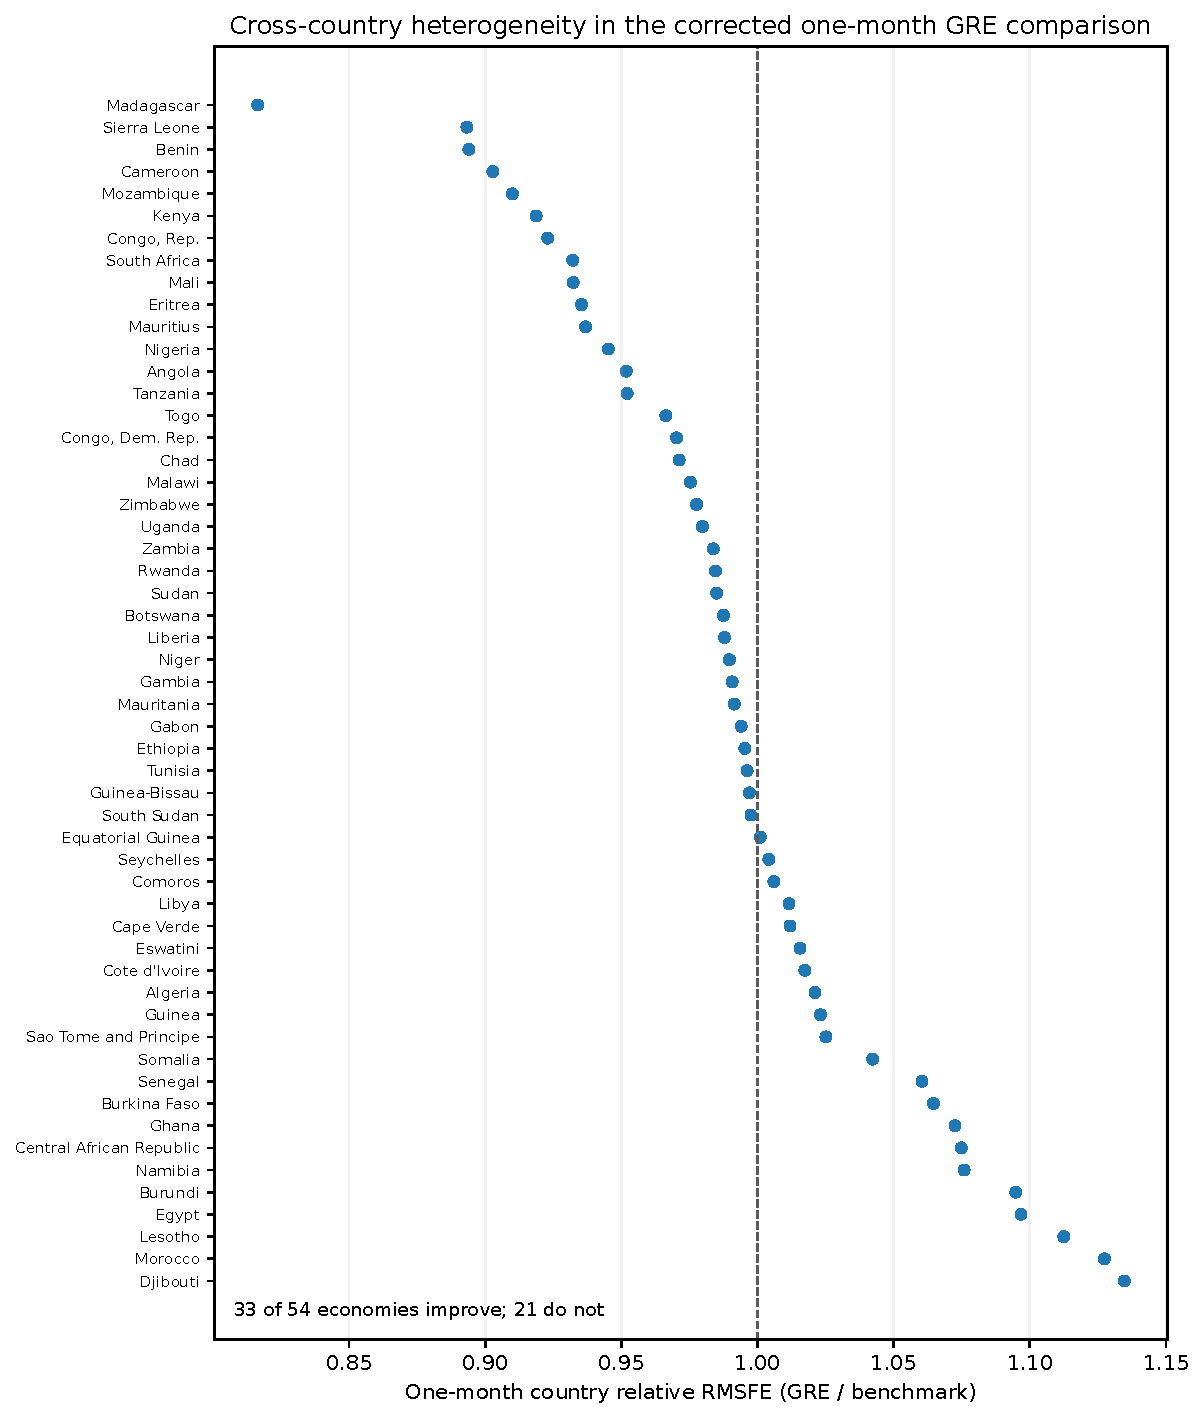
\includegraphics[width=0.88\textwidth,height=0.84\textheight,keepaspectratio]{Figure_Country_Heterogeneity.pdf}
\caption{Cross-country heterogeneity in the corrected one-month GRE comparison.}
\label{fig:country_heterogeneity}
\begin{singlespace}\footnotesize\textit{Notes:} Each point is a country's one-month RMSFE from the GRE-augmented model divided by the corresponding publication-lagged benchmark RMSFE. Values below one indicate lower country-level RMSFE with GRE.\end{singlespace}
\end{figure}

The corrected short-horizon evidence is also economically specific. Table~\ref{tab:comparator} replaces GRE with broad AERI, Inflation Risk, and FX/External Risk under the identical one-month forecast design. GRE is the only text signal that lowers both RMSFE and MAE relative to the common benchmark. Broad AERI raises RMSFE to 1.0024 times the benchmark, Inflation Risk raises it to 1.0153, and FX/External Risk is approximately neutral at 1.0003.

\begin{table}[htbp]
\centering\small
\caption{Domain-alignment comparators at the one-month forecast horizon}
\label{tab:comparator}
\resizebox{\textwidth}{!}{%
\begin{tabular}{lrrrrr}
\toprule
Text signal & RMSFE & Relative RMSFE & MAE & HAC CW $p$ & Two-way $p$ \\
\midrule
Growth/Real Economy (GRE) & 8.344 & 0.9964 & 5.385 & 0.0006 & 0.053 \\
Broad AERI & 8.394 & 1.0024 & 5.452 & 0.0003 & 0.238 \\
Inflation Risk & 8.503 & 1.0153 & 5.563 & 1.000 & 0.992 \\
FX/External Risk & 8.377 & 1.0003 & 5.430 & $<0.001$ & 0.208 \\
\bottomrule
\end{tabular}}
\vspace{0.35em}
\begin{minipage}{0.97\textwidth}\footnotesize\textit{Notes:} All signals augment the same publication-lagged benchmark (RMSFE $=8.375$, MAE $=5.441$). GRE is the only signal that lowers both RMSFE and MAE. Clark--West adjustment can be positive even when unadjusted forecast loss is slightly higher for a nested model, so domain-alignment interpretation uses the raw loss measures jointly with dependence-robust inference rather than the Clark--West $p$-value alone.\end{minipage}
\end{table}


The Clark--West adjustment is designed for nested-model predictive-accuracy testing and can be positive even when unadjusted MSE is marginally higher. This feature is visible for broad AERI and FX/External Risk. We therefore do not use isolated Clark--West $p$-values to claim that those signals improve forecasts. Domain alignment is assessed from the combination of raw RMSFE/MAE and dependence-aware inference. On that basis, GRE is the only member of the restricted comparison set with a favorable raw-loss profile.

\subsection{Mechanism and article-level measurement diagnostics}
A natural interpretation of the one-month result is that contemporaneous news is most useful when the conventional annual-information set is stale. Table~\ref{tab:staleness} tests that implication directly by splitting forecast origins before and after each assumed annual release month. Under the May rule, one-month relative RMSFE is 0.9925 in January--April origins and 0.9985 after the assumed release. Under the July rule, the corresponding ratios are 0.9937 and 1.0010. These two designs are consistent with a larger role for news when the latest annual benchmark is older.

\begin{table}[htbp]
\centering\scriptsize
\caption{One-month GRE performance before and after the assumed annual-data release month}
\label{tab:staleness}
\resizebox{\textwidth}{!}{%
\begin{tabular}{llrrrr}
\toprule
Release convention & Information state & Target months & Rel. RMSFE & Rel. MAE & HAC CW $p$ \\
\midrule
May & Stale pre-release & 24 & 0.9925 & 0.9804 & 0.0008 \\
May & Refreshed post-release & 48 & 0.9985 & 0.9947 & 0.0286 \\
July & Stale pre-release & 36 & 0.9937 & 0.9815 & 0.0001 \\
July & Refreshed post-release & 36 & 1.0010 & 0.9984 & 0.1432 \\
November & Stale pre-release & 60 & 0.9975 & 0.9907 & 0.0005 \\
November & Refreshed post-release & 12 & 0.9961 & 0.9926 & 0.0574 \\
\bottomrule
\end{tabular}}
\vspace{0.35em}
\begin{minipage}{0.97\textwidth}\footnotesize\textit{Notes:} ``Stale'' denotes forecast origins before the assumed release month in year $y+1$, when the most recent permitted annual GDP benchmark is one year older than it is after the release. The May and July conventions show substantially larger raw-loss gains in stale months. The November split has only 12 post-release target months and does not preserve the same RMSFE ordering. Formal stacked information-age and revision regressions are reported in the text and supplement and do not establish a monotonic causal mechanism.\end{minipage}
\end{table}


The mechanism evidence is not uniform, however. Under the deliberately conservative November convention, the stale-period RMSFE ratio is 0.9975 and the post-release ratio is 0.9961, although the post-release comparison contains only 12 target months. More formally, stacking the May, July, and November simulations and regressing target-month loss improvement on the age of the annual information set, with origin and release-convention effects, yields a positive but statistically weak coefficient ($p=0.625$ for raw loss and $p=0.539$ for Clark--West adjusted loss). GRE also does not significantly predict the revision from the publication-lagged current-growth estimate to final-vintage growth at the forecast origin: the coefficient on standardized GRE is $-0.073$ percentage points with two-way $p=0.765$. We therefore do not claim that GRE forecasts statistical revisions or that information age is a fully identified causal channel. The stale-month split is best read as a mechanism diagnostic that is supportive under the two less extreme release conventions but inconclusive overall.

The baseline signal uses the frozen article-scoring architecture. To test whether repeated identical stories materially drive the result, we use a separately reconstructed article archive in which exact decoded article bodies are collapsed within country-months before the pillar indices are recomputed. The reconstruction removes 497,091 records, or 2.33 percent of reconstructed article rows, including 186,379 cross-outlet copies. Original and deduplicated GRE have pooled Pearson correlation 0.969, rank correlation 0.981, and median within-country correlation 0.999.

\begin{table}[htbp]
\centering\small
\caption{Article-level exact-text deduplication sensitivity at the one-month horizon}
\label{tab:dedup_gre}
\resizebox{\textwidth}{!}{%
\begin{tabular}{lrrrrr}
\toprule
GRE construction & Rel. RMSFE & Rel. MAE & HAC CW $p$ & Two-way $p$ & $N$ \\
\midrule
Original GRE, common sample & 0.9964 & 0.9897 & 0.0006 & 0.053 & 3,886 \\
Exact-text-deduplicated GRE & 0.9969 & 0.9905 & 0.0017 & 0.068 & 3,886 \\
\bottomrule
\end{tabular}}
\vspace{0.35em}
\begin{minipage}{0.97\textwidth}\footnotesize\textit{Notes:} The reconstructed article archive removes 497,091 exact within-country-month duplicate records (2.33 percent of reconstructed records), including 186,379 cross-outlet copies, and recomputes the Growth/Real Economy pillar. The common-sample original and deduplicated GRE series have pooled Pearson correlation 0.969, rank correlation 0.981, and median within-country correlation 0.999. This exercise tests sensitivity to repeated identical text; it does not vary the lexicon, severity map, or emphasis coefficients.\end{minipage}
\end{table}


On the identical common forecast sample, the original GRE has one-month relative RMSFE 0.9964 and the deduplicated GRE 0.9969. Relative MAE is 0.9897 and 0.9905, respectively. The target-month HAC Clark--West values are 0.0006 and 0.0017. Exact-copy repetition therefore affects individual country-month scores but does not generate the direction of the short-horizon forecasting result. This is an article-level measurement sensitivity to the retained-record universe; it does not establish invariance to alternative dictionaries, severity tiers, or textual-emphasis coefficients.

\subsection{Data-rich benchmark and empirical boundary}
A stronger test of incremental information conditions on a genuinely data-rich conventional information set. We therefore build a wide panel containing up to 162 monthly series: publication-lagged GDP growth, inflation, and exchange-rate depreciation for each of the 54 economies. Variables with fewer than 24 observations in the March 2016--December 2018 calibration window or negligible variance are removed, leaving 159 series. Means, standard deviations, and PCA loadings are estimated only in this pre-evaluation window and then frozen. Six factors are retained because they are the minimum needed to explain more than 80 percent of calibration-sample variance (82.1 percent). Inflation and exchange-rate information is lagged by one month in the baseline factor exercise and by two months in a release-timing sensitivity. These macro series are also supplied final-vintage data without archived historical release vintages; the lagging conventions therefore reduce timing risk but do not convert the factor exercise into a genuine real-time-vintage benchmark.\footnote{The factor exercise should therefore be interpreted as a data-rich robustness boundary under conservative publication lags, not as a fully reconstructed vintage database. This distinction mirrors the treatment of annual GDP in the primary design.}

\begin{table}[htbp]
\centering\scriptsize
\caption{One-month GRE comparison against a wide macroeconomic factor benchmark}
\label{tab:wide_factor}
\resizebox{\textwidth}{!}{%
\begin{tabular}{lrrrrrr}
\toprule
Benchmark information & Benchmark RMSFE & +GRE RMSFE & Rel. RMSFE & Rel. MAE & HAC CW $p$ & Two-way $p$ \\
\midrule
Pooled AR, publication-lagged GDP lags & 8.375 & 8.344 & 0.9964 & 0.9897 & 0.0006 & 0.053 \\
Wide factors, macro variables lagged 1 month & 9.325 & 9.313 & 0.9987 & 0.9946 & 0.112 & 0.148 \\
Wide factors, macro variables lagged 2 months & 9.875 & 9.881 & 1.0006 & 0.9972 & 0.451 & 0.457 \\
\bottomrule
\end{tabular}}
\vspace{0.35em}
\begin{minipage}{0.97\textwidth}\footnotesize\textit{Notes:} The wide information set contains 162 candidate monthly series: publication-lagged GDP growth, inflation, and exchange-rate depreciation for 54 economies. Series with fewer than 24 observations in the 2016:03--2018:12 calibration window or negligible variance are removed, leaving 159. Means, standard deviations, and PCA loadings are frozen before evaluation. Six components are retained because they are the minimum needed to exceed 80 percent of pre-evaluation variance (82.1 percent). The wide factor benchmark is data-rich but has higher absolute RMSFE than the parsimonious AR benchmark. The inflation and exchange-rate series are supplied final-vintage macro data without archived release vintages, so one- and two-month lags are used as timing safeguards rather than claimed real-time vintages. GRE's small incremental improvement is not statistically significant against this benchmark.\end{minipage}
\end{table}


The factor exercise materially qualifies the empirical claim. The wide factor benchmark itself has higher absolute RMSFE than the parsimonious publication-lagged AR benchmark, illustrating that more conventional information is not automatically a stronger point forecast in this heterogeneous panel. Adding GRE to the one-month-lag factor specification lowers relative RMSFE to 0.9987 and relative MAE to 0.9946, but the HAC and two-way Clark--West values are 0.112 and 0.148. With a two-month macro lag, relative RMSFE is approximately one. Thus GRE does not deliver statistically persuasive incremental information once this wide factor augmentation is imposed. The surviving short-horizon result should therefore be interpreted as benchmark-dependent rather than as evidence that news dominates a rich conventional information set.

Figure~\ref{fig:release_benchmark} places the release-calendar robustness and the data-rich benchmark on the same one-month RMSFE scale. The three annual-release conventions yield similar favorable point estimates under the parsimonious benchmark, whereas the incremental advantage contracts toward one once the 159-series factor information set is imposed.

\begin{figure}[htbp]
\centering
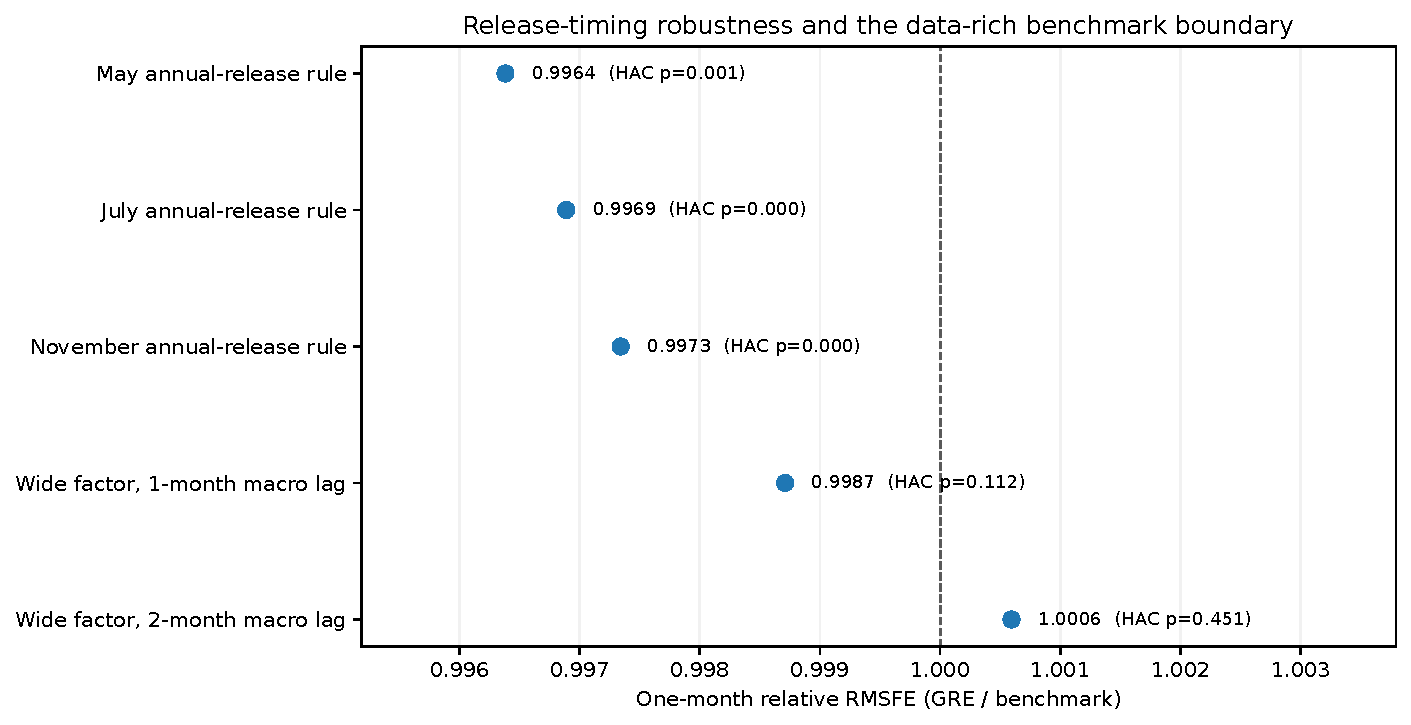
\includegraphics[width=0.90\textwidth]{Figure_Release_Benchmark_Boundary.pdf}
\caption{Release-timing robustness and the data-rich benchmark boundary at the one-month horizon.}
\label{fig:release_benchmark}
\begin{singlespace}\footnotesize\textit{Notes:} Points report relative RMSFE for GRE versus the corresponding benchmark. The first three rows vary the assumed annual GDP release month under the parsimonious publication-lagged benchmark. The final two rows augment the conventional information set with six principal components extracted from 159 retained macroeconomic series. Parenthetical values are target-month HAC Clark--West $p$-values.\end{singlespace}
\end{figure}

The one-month RMSFE improvement under the parsimonious benchmark is approximately 0.36 percent and the MAE improvement about 1.03 percent. These are modest effects. They would not justify a costly news-processing infrastructure if point forecasting were the only objective. Their operational relevance is more plausible for institutions that already maintain news pipelines for surveillance and can use GRE as a challenger variable between low-frequency statistical releases.

The methodological result is more consequential than the numerical gain. An apparently favorable long-horizon comparison disappears when target-information timing is enforced; the remaining short-horizon result survives release-calendar changes and exact-text deduplication but weakens against a wide macro factor benchmark and is not supported by a clean revision mechanism. The evidence therefore illustrates both sides of disciplined forecast evaluation: correcting leakage can overturn a result, while additional robustness tests can define precisely how much of the remaining evidence is portable across measurement and benchmark choices.
\section{Discussion and conclusion}
\subsection{What the evidence establishes}
The central result is methodological. A forecasting exercise that treats a final-vintage disaggregated path as both an ex post outcome and historically available lagged information does not reproduce the information set faced by the forecaster. The admissibility condition makes this point generally. The two Monte Carlo designs show why the sign of the distortion is not fixed: retrospective information can suppress a genuine short-horizon signal or, under a persistent-state stress calibration, produce an apparent long-horizon gain that disappears under publication timing. The African application then supplies a consequential empirical audit in which enforcing the information constraint reverses the original 12-month conclusion.

The application should therefore not be summarized as a new long-horizon GDP forecasting method. The retrospective 12-month GRE ratio of 0.9961 becomes 1.0048 once publication timing is enforced. The remaining one-month result is small, heterogeneous, and benchmark-dependent. It survives alternative annual-release conventions and exact-text deduplication, but the raw RMSFE bootstrap interval includes zero and the wide macro factor benchmark absorbs most of the incremental statistical evidence. The most defensible empirical interpretation is that monthly news can contain some short-horizon information when the conventional annual information set is sparse, but that this information is neither universal nor independent of the conventional benchmark.

The broader implication applies beyond text. Any forecasting study that converts low-frequency final-vintage macroeconomic data into a higher-frequency target should distinguish three objects: the realized evaluation target, the forecast-origin information set, and the data vintage used to construct each. If the target-construction operator uses future low-frequency benchmarks, the full constructed history should not be fed back into historical regressors. Origin-specific one-sided reconstruction, actual vintage data, or explicit publication-lag rules are preferable. At minimum, the retrospective and feasible-information results should be reported separately.

\subsection{Limitations and future validation}
The evaluation remains a publication-lagged final-vintage simulation rather than a fully real-time exercise. Future annual years are excluded from forecast-origin GDP histories and training outcomes are delayed, but annual observations treated as released still come from the final-vintage ``GDP (PPP)-WEO'' file and may contain later revisions. The monthly GDP target is also a constructed activity proxy whose within-year path depends on the Denton and extrapolation rules. A fully real-time extension using archived GDP vintages and country-specific release calendars would therefore provide the strongest additional validation.

The news measure is subject to a separate set of limitations. Exact-text deduplication shows that repeated identical stories do not drive the short-horizon result, but the analysis does not re-estimate alternative lexicons, severity rules, or emphasis weights, and the available human-coding workbook is a validation protocol rather than a completed label set. Arabic-only content may also be under-detected by the frozen English, French, and Portuguese activation dictionaries. These measurement limitations, together with the small and heterogeneous GRE gains and their attenuation under the 159-series factor benchmark, bound the empirical claim without altering the paper's central methodological result about target-information admissibility.

\paragraph{Funding.} This research did not receive any specific grant from funding agencies in the public, commercial, or not-for-profit sectors.

\paragraph{Data and code availability.} The replication package contains the author-supplied GDP workbook frozen on 13 September 2026, the cleaned annual ``GDP (PPP)-WEO'' extract, the final-vintage Denton outcome proxy, publication-lagged evaluation code and outputs, monthly GRE and comparator series, source registry, exact-text deduplication sensitivity, wide-factor benchmark, and the Monte Carlo code and outputs for the current-state, persistent-state stress, and pure-noise placebo designs introduced in Section~3. A separate retrospective folder preserves the earlier final-vintage-lag result solely for the target-information audit. The complete raw article archive is maintained separately because of its size.\footnote{The compact replication bundle contains the frozen monthly predictors and all files required to reproduce the reported forecast, simulation, factor, and deduplication results. The raw multi-million-record article archive is maintained separately to avoid making routine replication depend on transferring the full production corpus.}

\clearpage
\begin{thebibliography}{99}
\bibitem[Croushore and Stark(2001)]{croushorestark2001} Croushore, D., \& Stark, T. (2001). A real-time data set for macroeconomists. \emph{Journal of Econometrics}, 105, 111--130. https://doi.org/10.1016/S0304-4076(01)00072-0.
\bibitem[Croushore(2006)]{croushore2006} Croushore, D. (2006). Forecasting with real-time macroeconomic data. In G. Elliott, C. W. J. Granger, \& A. Timmermann (Eds.), \emph{Handbook of Economic Forecasting} (Vol. 1, pp. 961--982). Elsevier. https://doi.org/10.1016/S1574-0706(05)01017-7.
\bibitem[Ad{\"a}mmer et al.(2025)]{adaemmer2025} Ad{\"a}mmer, P., Pr{\"u}ser, J., \& Sch{\"u}ssler, R. A. (2025). Forecasting macroeconomic tail risk in real time: Do textual data add value? \emph{International Journal of Forecasting}, 41, 307--320. https://doi.org/10.1016/j.ijforecast.2024.05.007.
\bibitem[Ahir et al.(2022)]{ahir2022} Ahir, H., Bloom, N., \& Furceri, D. (2022). The World Uncertainty Index. NBER Working Paper 29763. https://doi.org/10.3386/w29763.
\bibitem[Ardia and Bluteau(2026)]{ardia2026} Ardia, D., \& Bluteau, K. (2026). Optimal text-based time-series indices. \emph{International Journal of Forecasting}, 42, 44--60. https://doi.org/10.1016/j.ijforecast.2025.07.003.
\bibitem[Abeyie(2026)]{abeyie2026} Abeyie, G. A. (2026). Beyond news headlines and TF-IDF: Enhancing text-based forecasting models with validated collocations and improved attention. \emph{International Journal of Forecasting}, 42, 752--773. https://doi.org/10.1016/j.ijforecast.2025.09.002.
\bibitem[Bae(2024)]{bae2024} Bae, J. (2024). Factor-augmented forecasting in big data. \emph{International Journal of Forecasting}, 40, 1660--1688. https://doi.org/10.1016/j.ijforecast.2024.02.004.
\bibitem[Denton(1971)]{denton1971} Denton, F. T. (1971). Adjustment of monthly or quarterly series to annual totals: An approach based on quadratic minimization. \emph{Journal of the American Statistical Association}, 66, 99--102. https://doi.org/10.1080/01621459.1971.10482227.
\bibitem[International Monetary Fund(2017)]{imfqna2017} International Monetary Fund. (2017). \emph{Quarterly National Accounts Manual: 2017 Edition}. Washington, DC: International Monetary Fund.
\bibitem[Baker et al.(2016)]{baker2016} Baker, S. R., Bloom, N., \& Davis, S. J. (2016). Measuring economic policy uncertainty. \emph{The Quarterly Journal of Economics}, 131, 1593--1636. https://doi.org/10.1093/qje/qjw024.
\bibitem[Ba{\'n}bura et al.(2013)]{banbura2013} Ba{\'n}bura, M., Giannone, D., Modugno, M., \& Reichlin, L. (2013). Now-casting and the real-time data flow. In G. Elliott \& A. Timmermann (Eds.), \emph{Handbook of Economic Forecasting} (Vol. 2A, pp. 195--237). Elsevier. https://doi.org/10.1016/B978-0-444-53683-9.00004-9.
\bibitem[Bok et al.(2018)]{bok2018} Bok, B., Caratelli, D., Giannone, D., Sbordone, A. M., \& Tambalotti, A. (2018). Macroeconomic nowcasting and forecasting with big data. \emph{Annual Review of Economics}, 10, 615--643. https://doi.org/10.1146/annurev-economics-080217-053214.
\bibitem[Caldara and Iacoviello(2022)]{caldara2022} Caldara, D., \& Iacoviello, M. (2022). Measuring geopolitical risk. \emph{American Economic Review}, 112, 1194--1225. https://doi.org/10.1257/aer.20191823.
\bibitem[Clark and West(2007)]{clarkwest2007} Clark, T. E., \& West, K. D. (2007). Approximately normal tests for equal predictive accuracy in nested models. \emph{Journal of Econometrics}, 138, 291--311. https://doi.org/10.1016/j.jeconom.2006.05.023.
\bibitem[Gentzkow et al.(2019)]{gentzkow2019} Gentzkow, M., Kelly, B., \& Taddy, M. (2019). Text as data. \emph{Journal of Economic Literature}, 57, 535--574. https://doi.org/10.1257/jel.20181020.
\bibitem[Giannone et al.(2008)]{giannone2008} Giannone, D., Reichlin, L., \& Small, D. (2008). Nowcasting: The real-time informational content of macroeconomic data. \emph{Journal of Monetary Economics}, 55, 665--676. https://doi.org/10.1016/j.jmoneco.2008.05.010.
\bibitem[Qu et al.(2024)]{qu2024} Qu, R., Timmermann, A., \& Zhu, Y. (2024). Comparing forecasting performance with panel data. \emph{International Journal of Forecasting}, 40, 918--941. https://doi.org/10.1016/j.ijforecast.2023.08.001.
\bibitem[Akgun et al.(2024)]{akgun2024} Akgun, O., Pirotte, A., Urga, G., \& Yang, Z. (2024). Equal predictive ability tests based on panel data with applications to OECD and IMF forecasts. \emph{International Journal of Forecasting}, 40, 202--228. https://doi.org/10.1016/j.ijforecast.2023.02.001.
\bibitem[Coroneo and Iacone(2025)]{coroneo2025} Coroneo, L., \& Iacone, F. (2025). Testing for equal predictive accuracy with strong dependence. \emph{International Journal of Forecasting}, 41, 1073--1092. https://doi.org/10.1016/j.ijforecast.2024.11.003.
\bibitem[Seo(2025)]{seo2025} Seo, B. (2025). Econometric forecasting using ubiquitous news text: Text-enhanced factor model. \emph{International Journal of Forecasting}, 41, 1055--1072. https://doi.org/10.1016/j.ijforecast.2024.11.001.
\bibitem[Stock and Watson(2002)]{stockwatson2002} Stock, J. H., \& Watson, M. W. (2002). Macroeconomic forecasting using diffusion indexes. \emph{Journal of Business \& Economic Statistics}, 20, 147--162. https://doi.org/10.1198/073500102317351921.
\bibitem[Stock and Watson(2004)]{stockwatson2004} Stock, J. H., \& Watson, M. W. (2004). Combination forecasts of output growth in a seven-country data set. \emph{Journal of Forecasting}, 23, 405--430. https://doi.org/10.1002/for.928.
\bibitem[Timmermann(2006)]{timmermann2006} Timmermann, A. (2006). Forecast combinations. In G. Elliott, C. W. J. Granger, \& A. Timmermann (Eds.), \emph{Handbook of Economic Forecasting} (Vol. 1, pp. 135--196). Elsevier. https://doi.org/10.1016/S1574-0706(05)01004-9.
\bibitem[Zheng et al.(2024)]{zheng2024} Zheng, T., Fan, X., Jin, W., \& Fang, K. (2024). Words or numbers? Macroeconomic nowcasting with textual and macroeconomic data. \emph{International Journal of Forecasting}, 40, 746--761. https://doi.org/10.1016/j.ijforecast.2023.05.006.
\end{thebibliography}
\end{document}
